Um den bestm\"oglichen Client f\"ur ein Spiel zu entwickeln, ist es von besonderer Bedeutung Fehler zu entfernen und stetig die Qualit\"at der Implementierung zu erh\"ohen.
Wir haben bereits zu Beginn festgestellt, dass es nur sehr schwer nachvollziehbar ist, abgeschlossene Spiele zu analysieren.
Wurde man nun durch fehlerhafte Z\"uge disqualifiziert, oder ist der Code bei einer bestimmten Stelle immer abgest\"urzt, war es sehr schwer diese Situation wiederherzustellen.
Zudem sind die aktuellen Informationen \"uber die Heuristik kaum aus gespielten Spielen herauszulesen.
Genau aus diesen Gr\"unden wurde die Software GameAnalyzer entwickelt.

\subsection{Rekonstruktion von Spielen}\label{subsec:rekonstruktion-von-spielen}
Ein wesentlicher Aspekt liegt darin ein gespieltes Spiel Schritt-f\"ur-Schritt nachspielen zu k\"onnen.
Das ist auch der erste wichtige Bestandteil dieser Software.
Wie man in Abbildung~\ref{fig:gameanalyze-start} sehen kann, wird gleich zu Beginn ein Spiel der gew\"ahlten Gruppe eingelesen und alle ausgew\"ahlten Z\"uge nachgeahmt.

\vspace{1em}
\begin{minipage}{\linewidth}
    \centering
    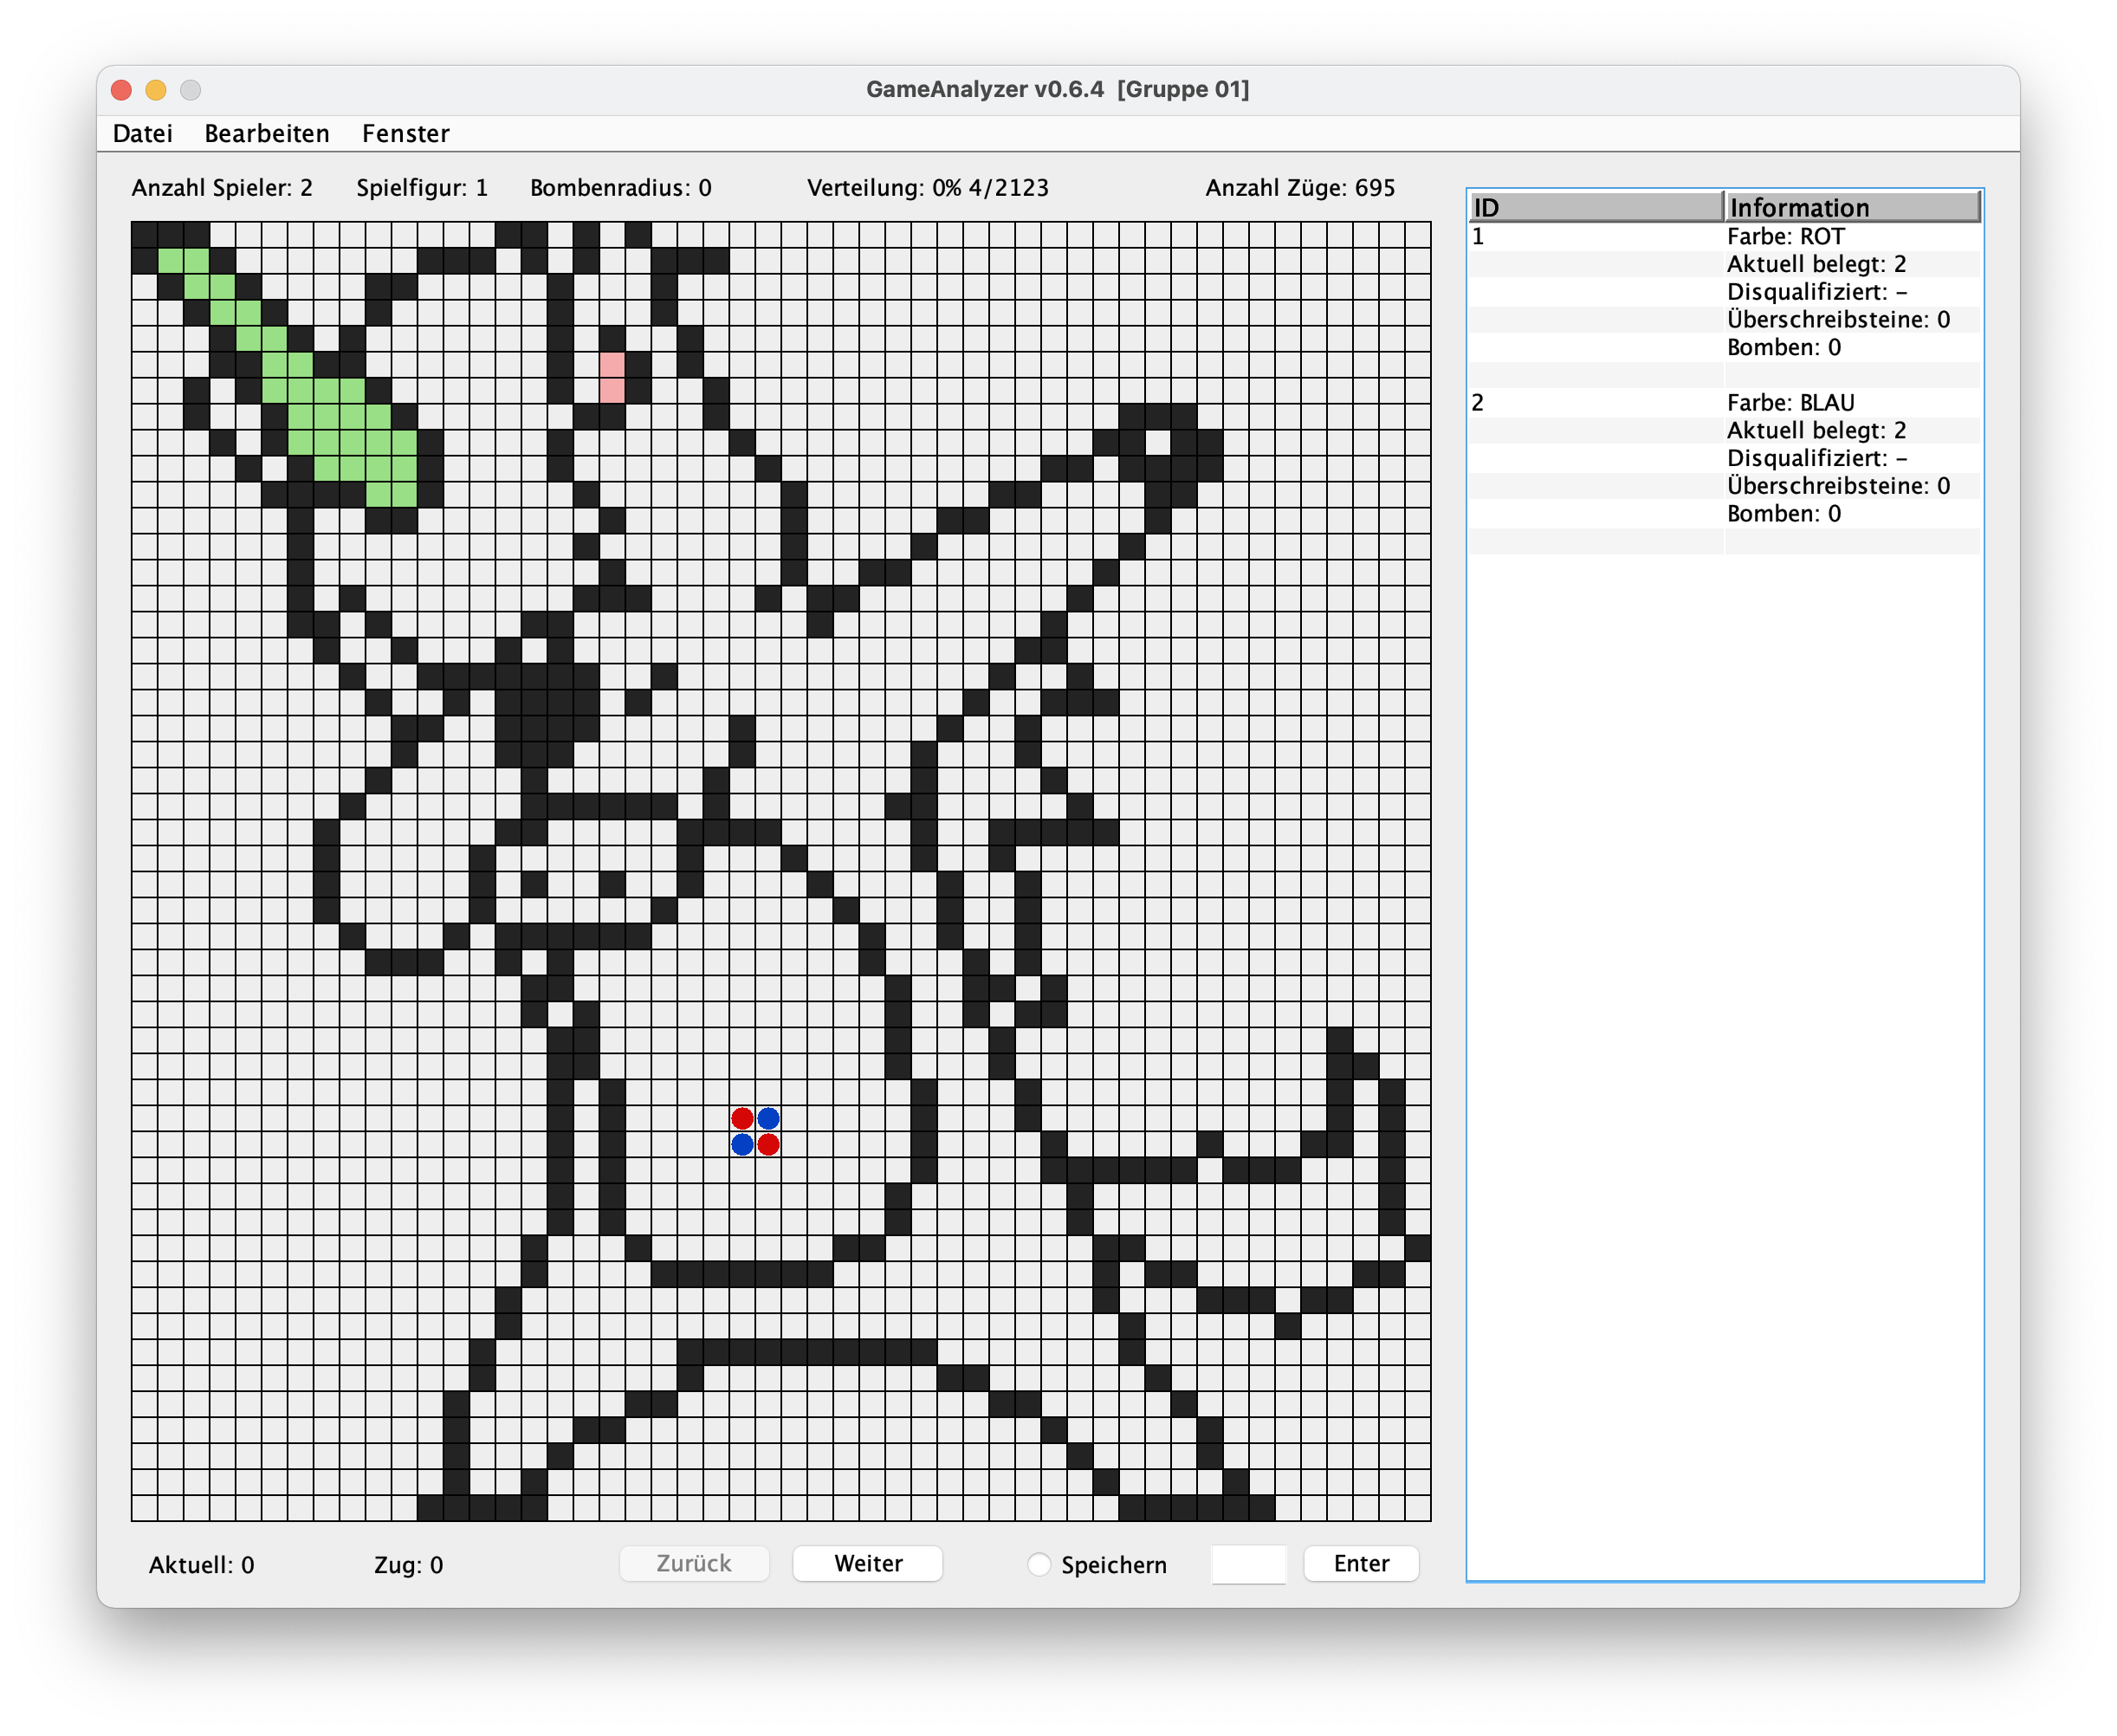
\includegraphics[width=0.7\linewidth]{pics/startscreen}
    \captionof{figure}[Startbildschirm GameAnalyze]{Startbildschirm GameAnalyze nach Auswahl einer Logdatei.}
    \label{fig:gameanalyze-start}
\end{minipage}

Mit den Tasten Weiter und Zur\"uck kann man das Spiel in beide Richtungen durchlaufen.
In der rechten Tabelle werden alle Spieler angezeigt.
Zudem kann man daran erkennen wie viele \"Uberschreibsteine, Bomben bzw.\ Spielsteine sie jeweils aktuell haben.
Ebenfalls ist zu sehen, welche Farbe sie haben und gegebenenfalls wann sie disqualifiziert wurden.
Man erh\"alt zudem Informationen dar\"uber, wie viele Spielz\"uge es gibt und wie viel Prozent an Spielsteinen aktuell belegt sind.
Zudem kann unter Datei $\rightarrow$ Exportieren der aktuelle Stand der Karte exportiert werden, damit die Karte mit dem gew\"unschten Spielstand dann wieder eingelesen werden kann.
Falls Transitionen existieren, k\"onnen diese unter Bearbeiten ein- bzw.\ ausgeschaltet werden.

\subsection{Anzeige erreichbarer Felder}\label{subsec:anzeige-erreichbarer-felder}
Damit keine Spielfelder betrachtet werden m\"ussen die auf dieser Karte garnicht erreichbar sind, haben wir einen MapAnalyzer entwickelt, der zu Beginn des Spieles unerreichbare Positionen aus der Karte herausrechnet.
Welche Felder erreichbar bzw.\ nicht erreichbar sind kann man sich ebenfalls anzeigen lassen.
Dazu geht man auf Fenster $\rightarrow$ Erreichbare Spielfelder.
Nun wird ein Fenster ge\"offnet, wie in Abbildung~\ref{fig:reachable-fields} zu sehen ist.

\vspace{1em}
\begin{minipage}{\linewidth}
    \centering
    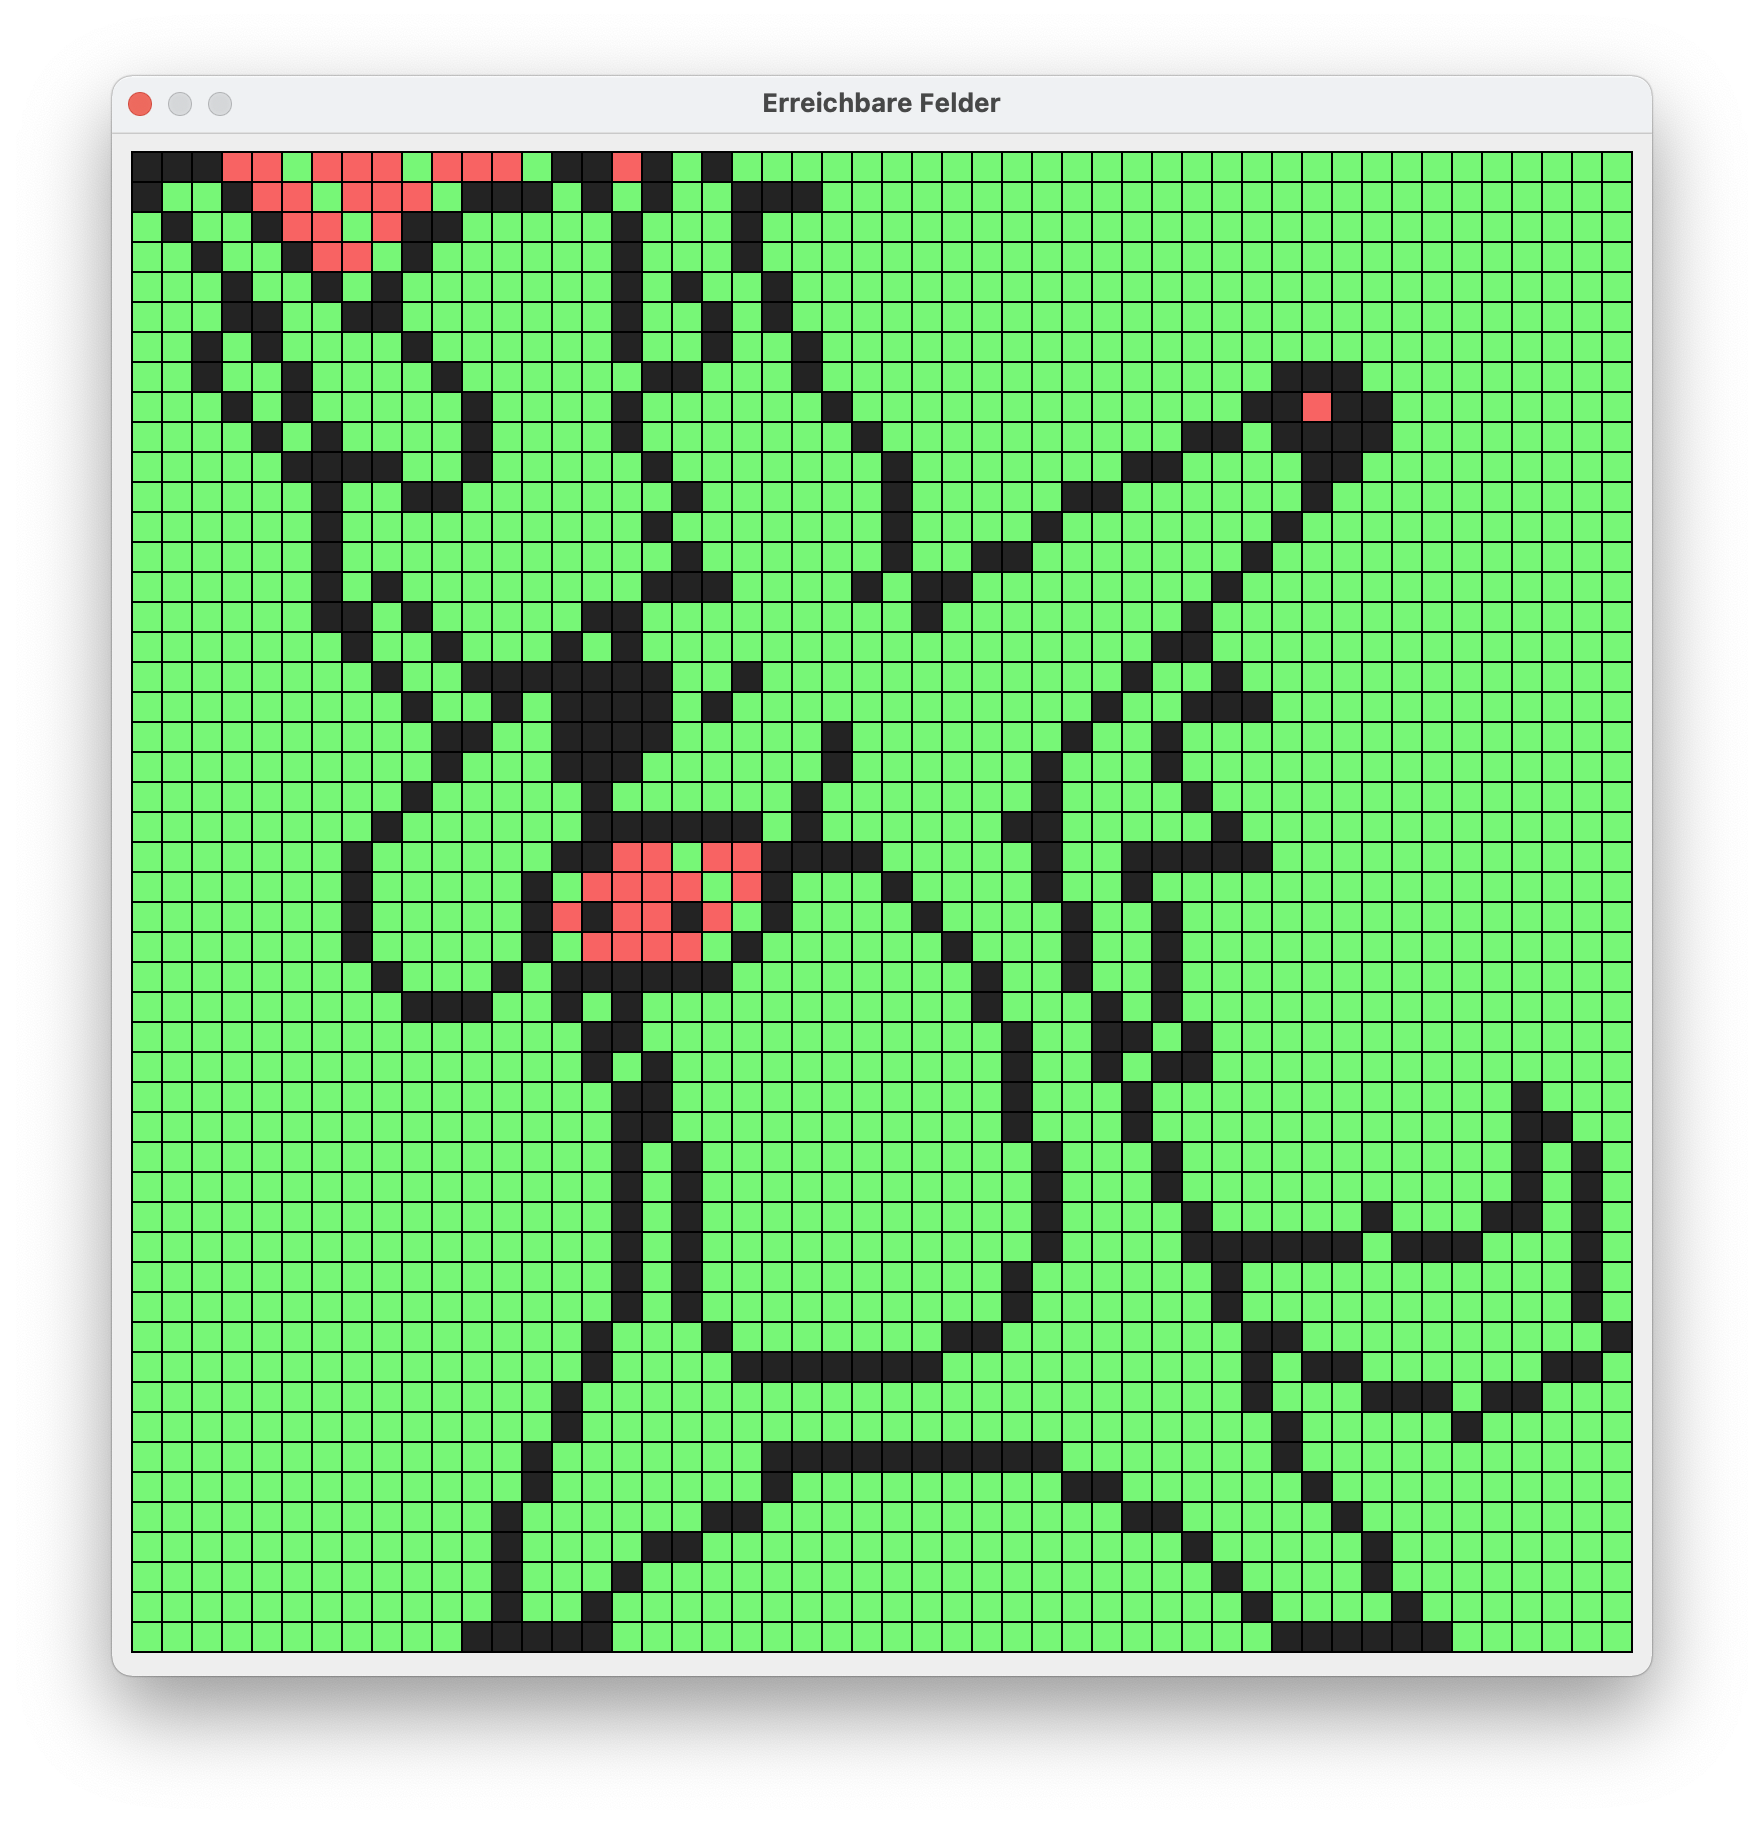
\includegraphics[width=0.7\linewidth]{pics/reachable-fields}
    \captionof{figure}[Anzeige unerreichbarer Felder]{Fenster um unerreichbare Felder anzuzeigen.}
    \label{fig:reachable-fields}
\end{minipage}

Schwarze Felder bedeuten, dass es sich hier um ein Loch handelt und dieses Feld somit generell nicht erreichbar ist.
Gr\"une Felder zeigen die Felder an, die w\"ahrend des Spieles erreichbar sind.
Was jedoch nicht bedeutet, dass sie erreicht werden m\"ussen.
Rote Felder symbolisieren, dass diese Felder w\"ahrend des gesamten Spieles definitiv nicht erreicht werden k\"onnen.

\subsection{Anzeigen detaillierter Statistiken}\label{subsec:anzeigen-detaillierter-statistiken}
Unter Fenster kann man sich die unterschiedlichen Statistiken anzeigen lassen.
Wie Sie in Abbildung~\ref{fig:heuristic} sehen k\"onnen, wird damit der gesamte Zustand eines Spielers w\"ahrend des Spieles angezeigt.
Dabei wird immer die aktuelle Implementierung verwendet.

\vspace{1em}
\begin{minipage}{\linewidth}
    \centering
    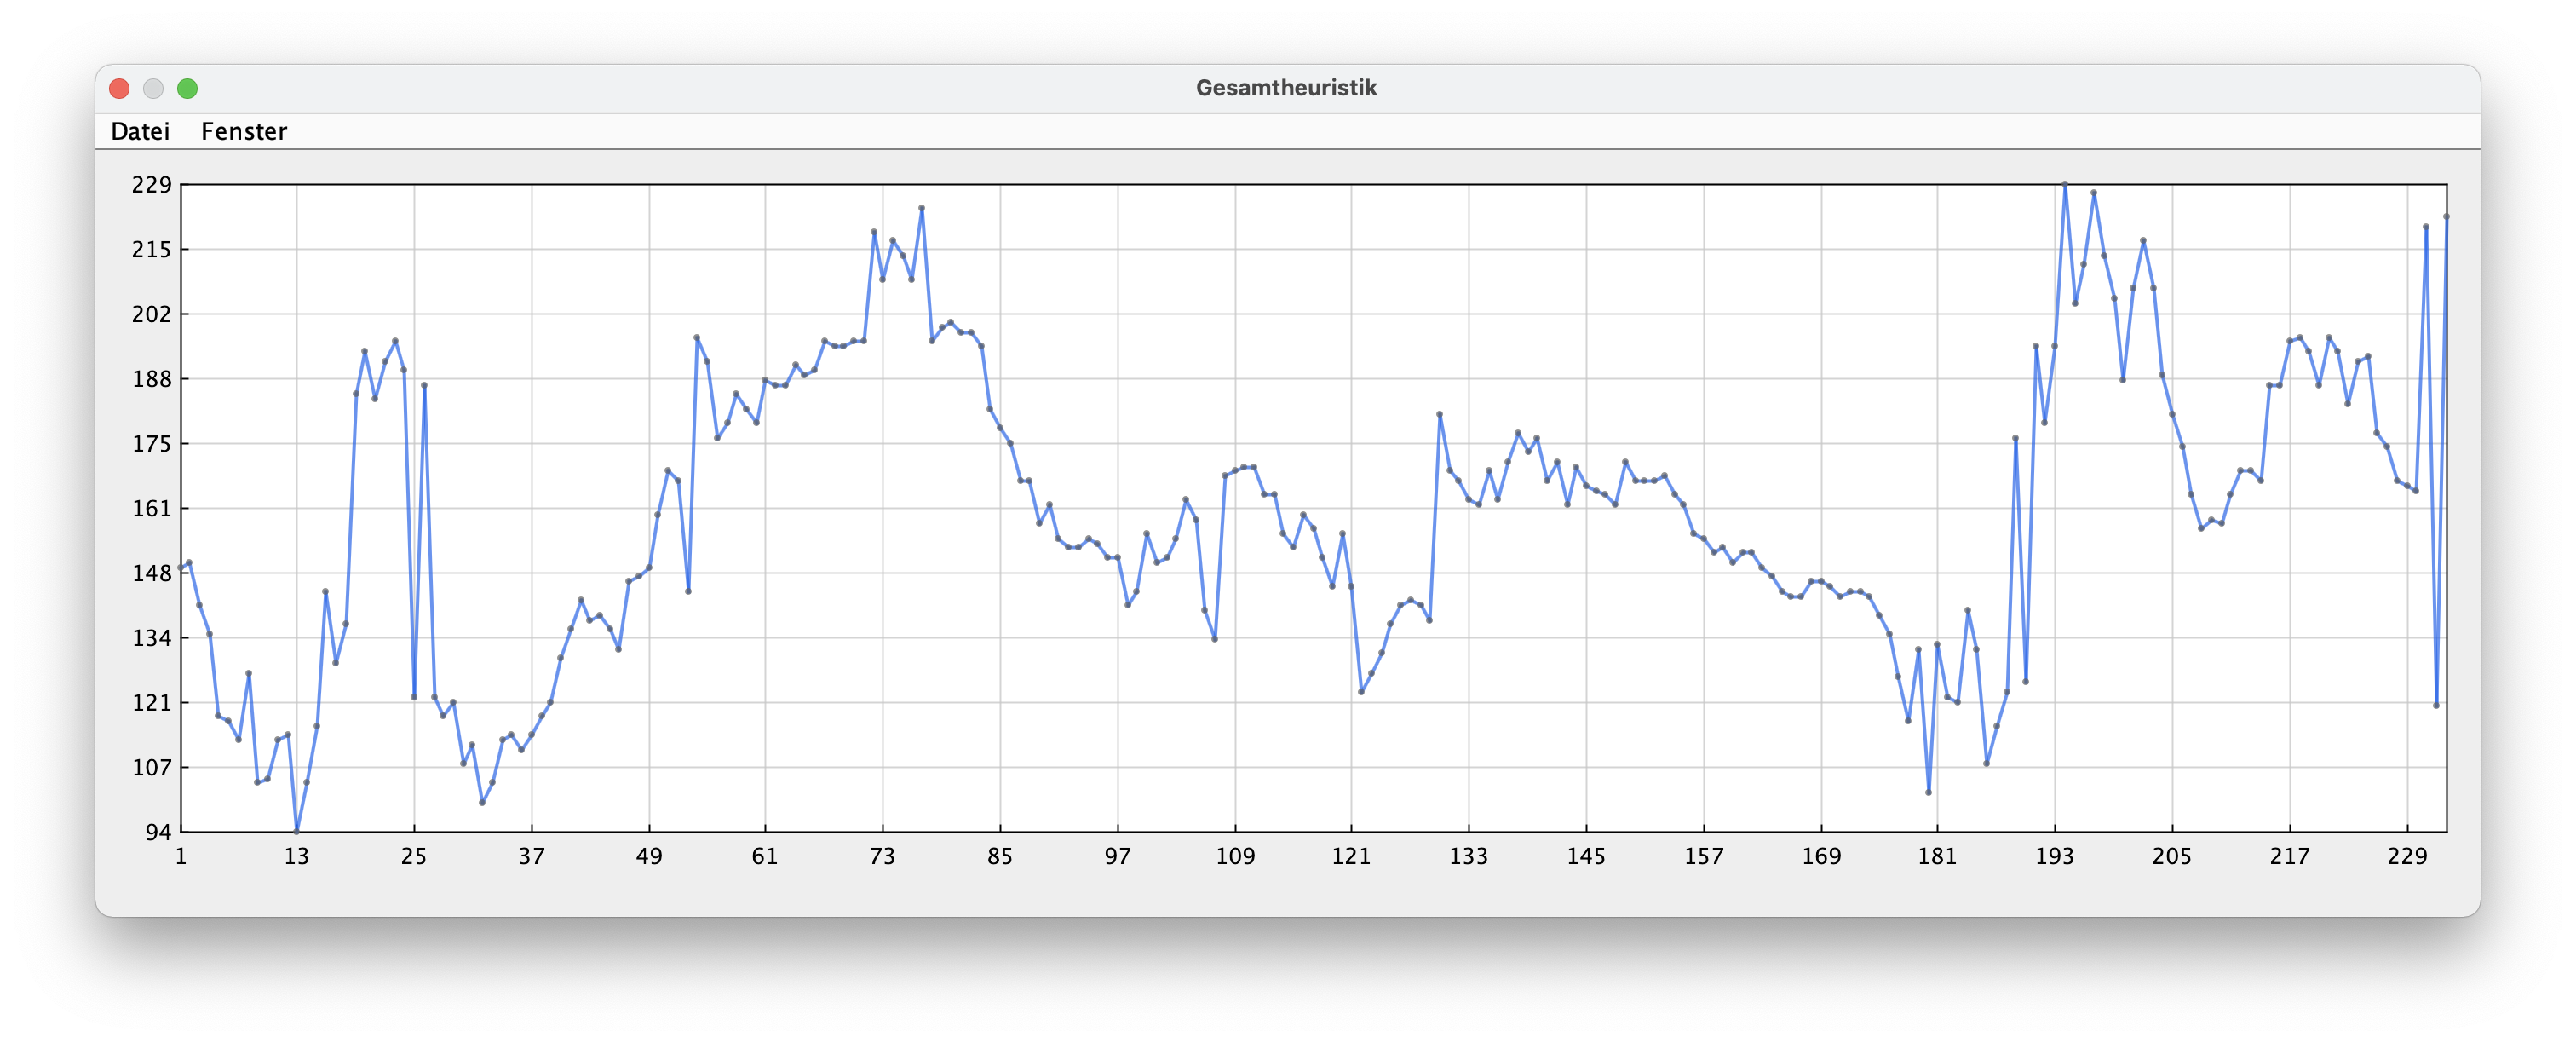
\includegraphics[width=0.8\linewidth]{pics/heuristic}
    \captionof{figure}[Grafik der Heuristik]{Fenster um aktuelle Heuristik anzuzeigen.}
    \label{fig:heuristic}
\end{minipage}

M\"ochte man Zust\"ande der Heuristik f\"ur sp\"ater speichern, kann man sich diese selbstverst\"andlich exportieren lassen und mit Grafiken in der Zukunft vergleichen.
Ein solcher Vergleich kann nat\"urlich auch dazu genutzt werden, um unterschiedliche Spieler bzw.\ Varianten miteinander in Relation zu setzen.
Dies haben sie bereits in Kapitel~\ref{subsubsec:vergleich-der-algorithmen} gesehen.

\subsection{Nutzen der Spielanalyse}\label{subsec:nutzen-der-spielanalyse}
Die Entwicklung der Spielanalyse war ein ziemlich zeit-kostenintensiver Prozess.
Es werden des \"Ofteren Spiele gegen andere Teams \"uber die Plattform Matchpoint gespielt.
Im Anschluss werden die Logdateien an die Gruppen verteilt, damit man eventuelle Abst\"urze finden oder auch generell den Spielverlauf anzeigen und verbessern kann.
Ein solches Turnier liefert gerne mal mehrere Hunderte Logfiles, die man sich am Besten alle genaustens anschauen sollte.
Diese Software tr\"agt wesentlich dazu bei, dass das f\"ur uns in \"uberschaubarer Zeit und noch dazu sehr detailliert m\"oglich ist.


\bigskip
\newpage